\documentclass[11pt, oneside]{article}   	% use "amsart" instead of "article" for AMSLaTeX format
\usepackage{geometry}                		% See geometry.pdf to learn the layout options. There are lots.
\usepackage{enumitem}
\usepackage{mathtools}

\geometry{letterpaper}                   		% ... or a4paper or a5paper or ... 
%\geometry{landscape}                		% Activate for rotated page geometry
%\usepackage[parfill]{parskip}    		% Activate to begin paragraphs with an empty line rather than an indent
\usepackage{graphicx}				% Use pdf, png, jpg, or eps§ with pdflatex; use eps in DVI mode
								% TeX will automatically convert eps --> pdf in pdflatex		
\usepackage{amssymb}
\usepackage{multicol}

\usepackage{xcolor}
\usepackage{textcomp}
\usepackage{subfigure}

%SetFonts

%SetFonts
% code listing settings
\usepackage{listings}
\lstset{
    language=Python,
    basicstyle=\ttfamily\small,
    aboveskip={1.0\baselineskip},
    belowskip={1.0\baselineskip},
    columns=fixed,
    extendedchars=true,
    breaklines=true,
    tabsize=4,
    prebreak=\raisebox{0ex}[0ex][0ex]{\ensuremath{\hookleftarrow}},
    frame=lines,
    showtabs=false,
    showspaces=false,
    showstringspaces=false,
    keywordstyle=\color[rgb]{0.627,0.126,0.941},
    commentstyle=\color[rgb]{0.133,0.545,0.133},
    stringstyle=\color[rgb]{01,0,0},
    numbers=left,
    numberstyle=\small,
    stepnumber=1,
    numbersep=10pt,
    captionpos=t,
    escapeinside={\%*}{*)}
}


\title{Project Report}
\author{Omar Ghaleb\\
COMP 5107}
\date{}							% Activate to display a given date or no date

\begin{document}
\renewcommand\thesubsection{\alph{subsection}.}
\maketitle
%\section{}
%\subsection{}
%\begin{enumerate}[label=\alph*)]
%	\item First item
%\end{enumerate}
\section*{Problem}
The idea of the project is to create a pattern classifier based on different methods and types of classifier on a selected dataset. In the project we created four main different classifiers:
\begin{itemize}
	\item Quadratic: Maximum Likelihood(ML), Bayesian(BL) and Parzen Window
	\item K-Nearest Neighbours
	\item Fisher's Discriminant 
	\item Ho-Kashyap
\end{itemize}
For testing the classifiers, five-cross validation was used.
The code is available on the following link:
https://github.com/omaramin1992/comp5107 

\section*{Dataset}
The dataset selected is used to classify different types of glass. The reason for this is that identifying the type of glass helps in criminology. The data had no empty values thus it did not need to be cleaned. The data set contained 9 features(6 were selected which are Refractive index, Magnesium, Aluminum, Potassium, Barium and Iron) and two main classes and 9 subclasses. For our project we worked with the whole dataset as two main classes only which are (window or non-window) or class1 and class2 respectively. In the project, the data were projected on the first and second dimensions only (x1-x2).

The data was the normalized since the scales were far off from each other and affected the classification behaviour, hence, it was needed to make the scales similar by normalizing the data between 0 and 1. In Figure~\ref{fig:data-points}, we can see the effect of normalizing the data.

\begin{figure}
\begin{center}
	\subfigure[Before Normalizing ]{
	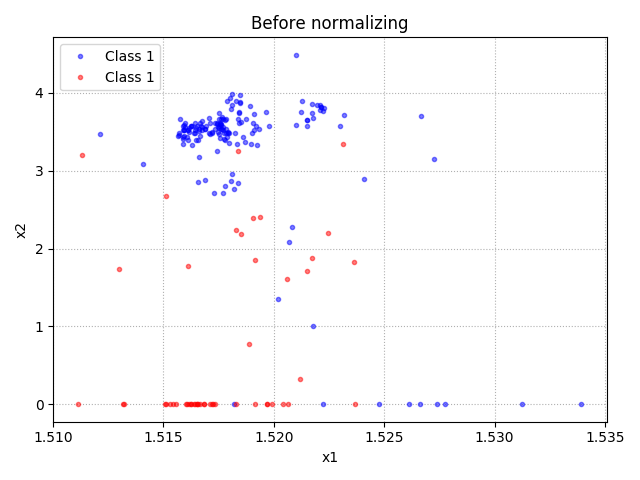
\includegraphics[width=0.45\textwidth]{plots/data-before-norm.png}
	\label{absorbing}
	}
	\subfigure[After Normalizing]{
	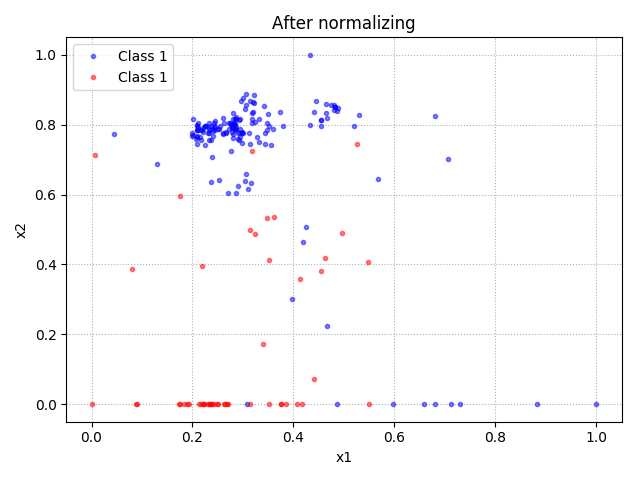
\includegraphics[width=0.45\textwidth]{plots/data-after-norm.png}
	\label{absorbing}
	}
\end{center}
\caption{Data Points in x1-x2 dimensions}
\label{fig:data-points}
\end{figure}

One problem with the data, and we will see the effect of that, is how close both classes are to each other as they both have very close means. Another problem is that the first class (window) consists of 3 times the instances of the other class(non-window).

\section*{Classifiers}

Below, we are going to go through our different classifiers that we created for this dataset.

\subsection{Quadratic Classifiers}

First, we are going to talk about the quadratic classifiers (ML, BL, Parzen).

\subsubsection*{Maximum Likelihood (ML)}
We use the ML to estimate the parameters of the quadratic classifier, $M$ and $\Sigma_{X_1}$, for each class by using the equation:
$$ \hat{M}= \frac{1}{N} \sum_{i=1}^{N} x_i, \quad\quad \hat{\Sigma}=	 \frac{1}{N} \sum_{i=1}^{N}[X_i-\hat{M}][X_i-\hat{M}]^T$$
And the resulting means were the following for each class:
$$\hat{M_1} = \begin{bmatrix}
0.32673694 \\ 0.73383251 \\ 0.30892724 \\ 0.07688964 \\ 0.00946538 \\ 0.13256345
\end{bmatrix},\quad \hat{M_2} = \begin{bmatrix}
0.28480435 \\ 0.16341325 \\ 0.52232606 \\ 0.09011398 \\ 0.20292561 \\ 0.04536717
\end{bmatrix}$$
  and covariance matrices as follows: 
  $$\Sigma_{X_1} = \begin{bmatrix}
  0.0178 &-0.0149& -0.0061& -0.00291&  0.00349 & 0.0028\\
 -0.0149&  0.0388&  0.0001&  0.00149& -0.00454 &-0.0053\\
 -0.0061 & 0.0001 & 0.0101 & 0.00251 & 0.00161 & 0.0010\\
 -0.0029 & 0.0014 & 0.0025 & 0.00123  &0.00003 & 0.0005\\
  0.0034 &-0.0045 & 0.0016 & 0.00003  &0.00643 & 0.0027\\
  0.0028 &-0.0053 & 0.0010 & 0.00051  &0.00270 & 0.0378
\end{bmatrix},$$ $$\Sigma_{X_2} = \begin{bmatrix}
  0.0159 & 0.0075 &-0.0086 &-0.0072& -0.0050 & 0.0033\\
  0.0075 & 0.0589 &-0.0082 & 0.0017& -0.0056 & 0.0004\\
 -0.0086 &-0.0082 & 0.0340 & 0.0120&  0.0125 & 0.0015\\
  0.0072 & 0.0017 & 0.0120 & 0.0419& -0.0050 &-0.0014\\
 -0.0050 &-0.0056 & 0.0125 &-0.0050&  0.0549 &-0.0032\\
  0.0033 & 0.0004 & 0.0015 &-0.0014& -0.0032 & 0.0257
\end{bmatrix}$$

These values estimate parameter are gonna be our basis for any actual values needed or calculations that needs the real covariances(such as BL).
Once we estimated the parameters, we were able to estimate the discriminant function and plot it in $(x1-x2)$ dimensions, as in Figure~\ref{fig:ml-disc-func}, before and after diagonalizing the data.

After that we diagonalize the data and get the corresponding covariance matrices. For class 1 it becomes the identity matrix $I$ and for class 2 is the diagonal matrix of the following:
$$\Sigma_{X_2} = \begin{bmatrix}
  82.8012 & 11.2717 & 4.4823 & 3.0525 & 0.4904 & 0.6506
\end{bmatrix}$$
After that, we tested our classifier using five-cross validation and we got an average accuracy of 78.55\%. (97.57\% for class 1 and 17.81\% for class 2) for both before and after diagonalizing the data. We can see that the accuracy is skewed towards the first class more and that i believe due to three main reasons:
\begin{itemize}
	\item The data means are close to each other
	\item The number of instance in each each are significantly different as class 1 is three times class 2
	\item The correlation between the selected features and the classses
\end{itemize}

\begin{figure}
\begin{center}
	\subfigure[Before Diagonalizing ]{
	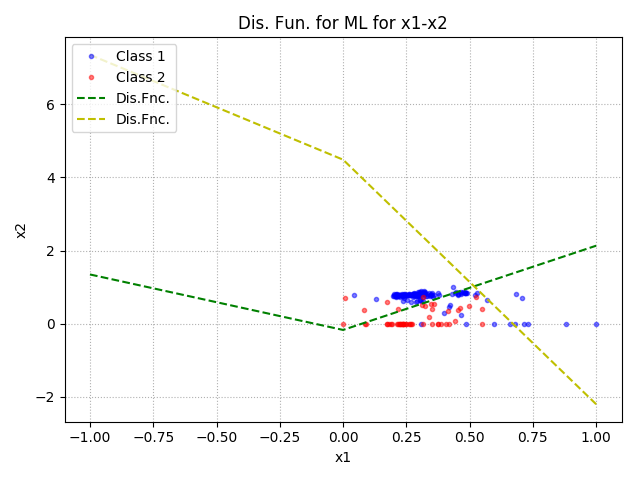
\includegraphics[width=0.45\textwidth]{plots/ml-disc-func.png}
	\label{absorbing}
	}
	\subfigure[After Diagonalizing]{
	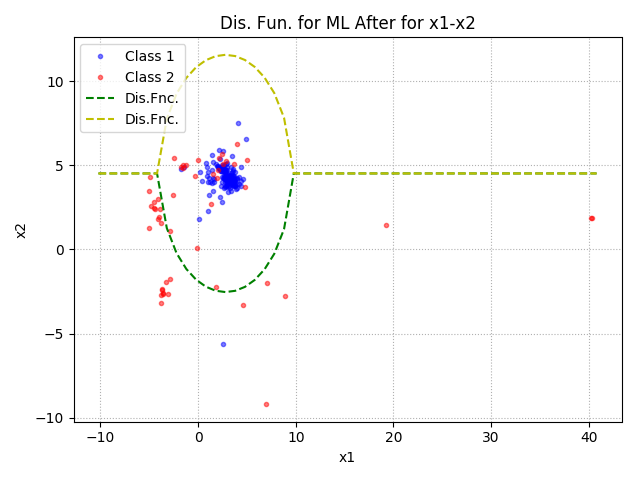
\includegraphics[width=0.45\textwidth]{plots/ml-disc-func-diag.png}
	\label{absorbing}
	}
\end{center}
\caption{ML Disc. Func. in x1-x2}
\label{fig:ml-disc-func}
\end{figure}

\subsubsection*{Bayesian Learning (BL)}
Next, we are going to estimate the means using BL method. In the calculating of the mean we used the following equation:
$$\left(m\right)_n=\frac{1}{n}\Sigma\left[\frac{1}{n}\Sigma+\Sigma_0\right]^{-1}m_0+\Sigma_0\left[\frac{1}{n}\Sigma+\Sigma_0\right]^{-1}\left(\frac{1}{n}\sum_{j=1}^{n}x_j\right)$$

In the above equation, we used the estimated covariance from ML as the actual covariance in calculating the mean. Since we used that covariance, we had the resulting estimate mean pretty close with high precision to ML estimates.
$$\hat{M_1} = \begin{bmatrix}
0.32677967 \\ 0.73378739 \\ 0.30897436 \\ 0.07690064 \\ 0.00953297 \\ 0.13279159
\end{bmatrix},\quad \hat{M_2} = \begin{bmatrix}
0.28492792 \\ 0.16435958 \\ 0.52282895 \\ 0.09079785 \\ 0.20358894 \\ 0.04584223
\end{bmatrix}$$

Then we used these estimates to calculate the discriminant function which resulted in a similar result as the ML as it is shown in Figure~\ref{fig:bl-disc-func}.

\begin{figure}
\begin{center}
	\subfigure[Before Diagonalizing]{
	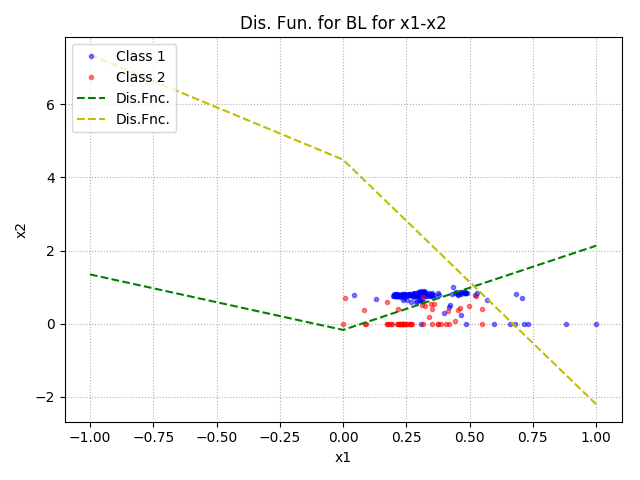
\includegraphics[width=0.45\textwidth]{plots/bl-disc-func.png}
	\label{absorbing}
	}
	\subfigure[After Diagonalizing]{
	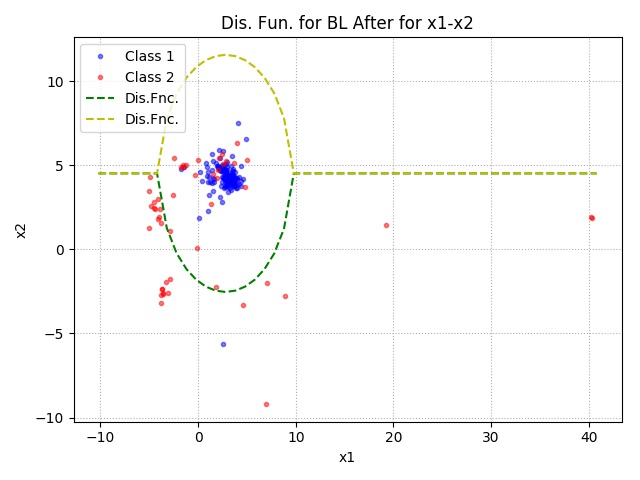
\includegraphics[width=0.45\textwidth]{plots/bl-disc-func-diag.png}
	\label{absorbing}
	}
\end{center}
\caption{BL Disc. Func. in x1-x2}
\label{fig:bl-disc-func}
\end{figure}

Since we got the same discriminant function(DF), in testing our DF, we got the same results are ML with an accuracy of 78.554\% for both before and after diagonalizing the data.

\subsubsection*{Parzen Window}
Next we use the Parzen window method to estimate the one feature only as requested and we used that to calculate the mean (estimate the density function) of the first feature (dimension). In Figure~\ref{fig:parzen} we can see the estimated mean for the first dimension for both classes how they are very close to each other. Parzen estimated means for all dimensions:
$$\hat{M_1} = \begin{bmatrix}
0.32673694 \\ 0.73383251 \\ 0.30892724 \\ 0.07688964 \\ 0.00946538 \\ 0.13256345
\end{bmatrix},\quad \hat{M_2} = \begin{bmatrix}
0.28480435 \\ 0.16341325 \\ 0.52232606 \\ 0.09011398 \\ 0.20292561 \\ 0.04536717
\end{bmatrix}$$

\begin{figure}
\begin{center}
	\subfigure{
	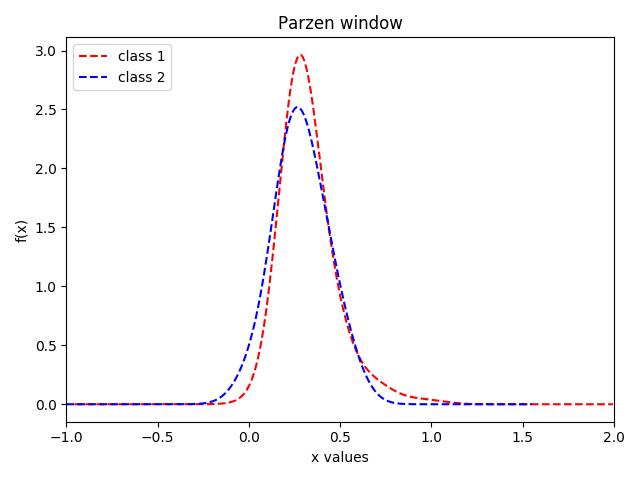
\includegraphics[width=0.45\textwidth]{plots/parzen-x1.png}
	\label{absorbing}
	}
\end{center}
\caption{Parzen Window}
\label{fig:parzen}
\end{figure}

\subsection{K-Nearest Neighbours Classifier}
Next, we used the k-nearest neighbours classifier to classify the data. In our case we used $k=5$ and the algorithm calculates the distances between the test point and all other training points and takes the closest five points and votes on the majority of the classes of these points. Then the testing point is classified according to the majority class.

Using K-NN, we reached the maximum accuracy we had for the data with a 90.18\% accuracy before diagonalizing and and accuracy of 85.89\% after diagonalizing the data. (Code is available online on the link provided in the beginning).

\subsection{Fisher's Discriminant Classifier}
Then, we used the concept of Fisher's Discriminant to classify the data by finding a hyperplane that the point can be projected on and then find the linear classifier that can classify the data as accurate as possible.
We calculated the vector $W$ that represents the plane that the points will be projected on:
$$W = \begin{bmatrix}
0.6697 \\ 5.5320 \\ -3.4231 \\ 0.4729 \\ -1.3701 \\ 1.871
\end{bmatrix}$$

And by using this transforming vector we get the points projected as in Figure~\ref{fig:fishers-disc} and we calculated the points of the discriminant function on that plane by solving the equation for one dimension instead of $d$ dimensions. After transforming the data the first and second class have means of 3.49242 and -0.84373 respectively.

\begin{figure}
\begin{center}
	\subfigure[Before Diagonalizing]{
	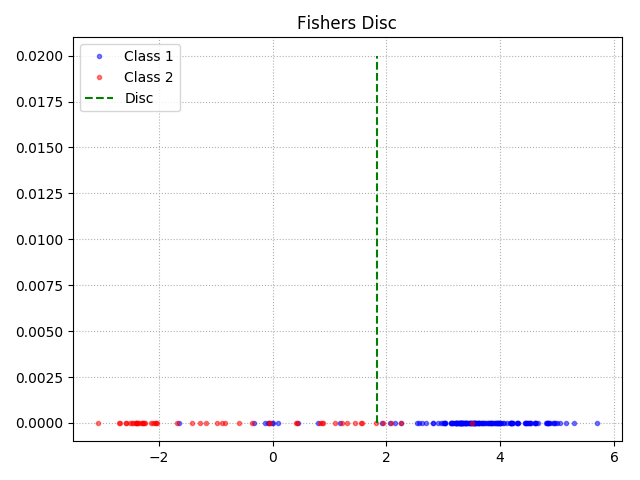
\includegraphics[width=0.45\textwidth]{plots/fishers-disc.png}
	\label{absorbing}
	}
	\subfigure[After Diagonalizing]{
	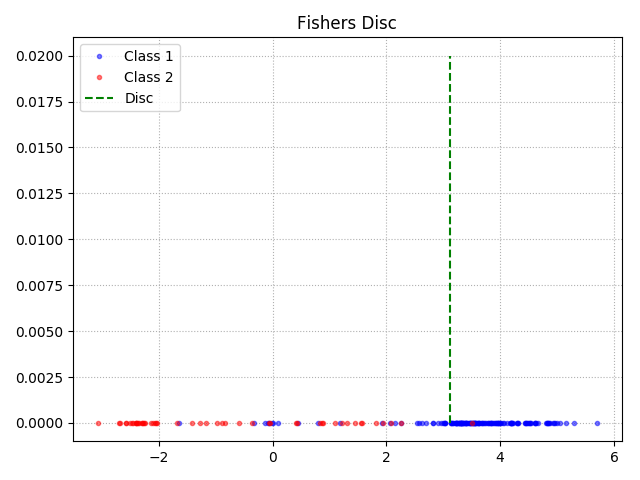
\includegraphics[width=0.45\textwidth]{plots/fishers-disc-diag.png}
	\label{absorbing}
	}
\end{center}
\caption{Fishers Discriminant}
\label{fig:fishers-disc}
\end{figure}

By testing the linear classifier, we got an accuracy of 88.825\% before diagonalizing and 88.8251\% which is the same accuracy after diagonalizing.

\subsection{Ho-Kashyap Classifier}
In ho-kashyap, a linear classifier is created based on the points only by using the concept of gradient decent. The algorithm for it is in Listing 1

\begin{lstlisting} [label={list:first},caption=Ho-Kashyap Code]
def ho_kashyap(class1_data, class2_data):
    class1_ones = np.ones(len(class1_data[0]))
    class2_ones = np.ones(len(class2_data[0]))

    y1 = np.array(class1_data)
    y2 = np.array(class2_data)

    y1 = np.insert(y1, 0, class1_ones, axis=0)
    y2 = np.insert(y2, 0, class2_ones, axis=0)

    y1 = y1.transpose()
    y2 = -1 * y2.transpose()

    y = np.append(y1, y2, axis=0)

    a = np.ones((len(y[0]), 1))
    b = np.ones((len(y), 1))

    lr = 0.9  # learning rate
    i = 0
    e = y @ a - b
    e1 = np.linalg.norm(e)

    for i in range(400):
        e = y @ a - b
        b = b + lr * (e - np.abs(e))
        a = np.linalg.inv(y.transpose() @ y) @ y.transpose() @ b
        e1 = np.linalg.norm(e)
        i = i + 1

    return a, b
\end{lstlisting}

By using this method we solve for $A$ and $B$ until it converges and since the classes are not linearly separable, it will not find a line that separates them completely. and by updating the weights $A$, we reach an $A$ and $B$ such that the error is minimized.

The testing of the classifier was tested using same method used before, five-cross validation, and the accuracy before diagonalizing was 85.675\% and after diagonalizing 78.6424\%.

\section*{Improvements}
To make this system a full pattern classification system, some of the class handling is meant to deal with only two classes and that could be extended to include multiple classes classification. It can also include a way of cleaning the data by removing outliers and removing the noisy data and that could help create a better classifier.  
\end{document}  








